\chapter{Reinforcement Learning for Surgical Tensioning}

\section{Introduction}
Robotic surgical assistants (RSAs), such as Intuitive Surgical's da Vinci, facilitate precise minimally invasive surgery~\cite{veldkamp2005laparoscopic}. These robots currently operate under pure tele-operation control, but introducing assistive autonomy has potential to improve surgical training, assist surgeons, reduce fatigue, and facilitate tele-surgery.
For example, when cutting thin tissue with surgical scissors, a surgeon may use a second or even a third tool to pin down and fixture the tissue.
This technique, called tensioning (also called traction), adds additional constraints on the material to prevent deformations during the cutting from drastically changing the position of the desired cutting path.
The optimal direction and magnitude of the tensioning force changes as the cutting progresses, and these forces must adapt to any deformations that occur. 
However, practically, the surgeon's tensioning policy is often sub-optimal because: (1) surgeon can automatically manipulate only two of the tools at once leaving any third arm stationary, and (2) asymmetric multilateral tasks (arms doing different procedures) are known to be challenging without significant training with the tele-operative system.

Therefore, it would be beneficial to automatically synthesize tensioning policies to best assist an open loop cutting trajectory. The first challenge is modeling the dynamics of cutting and tensioning. One way to model deformable sheets is with a 3-dimensional mass-spring-damper network. A sheet is a planar graph of point masses connected by damped springs at edges. $k$ of the point masses are constrained to be fixed at a particular 3D location, i.e., they are tensioned, and the positions of the remaining masses is determined by the dynamics induced these constraints. At each time step, the constraint can be moved to a new location. Cutting is modeled by removing a single edge in the graph at each time-step.  For $k$ assistive arms, the optimization objective is to plan  sequence of $k$ movable boundary value constraints to maximize cutting accuracy.

In prior work, we designed a tensioning planner using Trust Region Policy Optimization (TRPO) over the model to simulate the effect of different tensions and find a tensioning policy to assist a given cutting trajectory. 
The planner optimized was the final symmetric difference between a perfectly cut contour and the actual cut.
The learned policy can assist both human surgeons~\cite{reiley2010motion} and automated surgical cutting procedures to improve the reliability and accuracy of surgical cutting~\cite{swirl2016,murali2015learning}.
While initial results suggest that this adaptive policy is effective ($43.3\pm8.6\%$ better than a fixed-policy baseline over 17 contours), each new contour required expensive training of a new policy (approximately 50,000 rollouts). 
More efficient policy search techniques are required if we want to effectively assist a human surgeon seamlessly during a procedure.

One clear point for improvement is actually using the underlying simulation model to intelligently initialize TRPO.
The key challenge is that the objective the TRPO optimizes is non-convex and the system is non-linear.
This paper explores whether it is possible to linearize the system locally and solve for a quadratic greedy objective as a proxy.
This solution serves as an initialization which TRPO will further refine.
Our initial results suggest that the analytic model is within 25\% of the final reward of TRPO achieves on three curves.
This serves as a good initialization which significantly improves the convergence of TRPO.


\section{Related Work}
Nienhuys and Van Der Stappen proposed the seminal work on modeling cutting with finite-element mesh models~\cite{nienhuys2001surgery}.
This work led to a bevy of follow-on work in robotics and graphics modeling the cutting problem, especially in the context of surgical simulation~\cite{bielser2004state, sifakis2007arbitrary, mendoza2003simulating, steinemann2006hybrid}.
In parallel, the graphics community studied fabric modeling with similar finite-element techniques~\cite{gale2016patterning, brookes16tearable}.
In our prior work, we implemented such an approach for the Pattern Cutting task in the Fundamentals of Laparoscopic Surgery (FLS)~\cite{thananjeyanmultilateral}.
This paper is inspired by the challenges noticed in our prior work, namely, that state-estimation of a deformable object when there are occlusions is very challenging. 
Therefore, we investigate whether synthesizing a tensioning plan \emph{a priori} can mitigate this problem.

Manipulation of deformable materials, particularly cutting, is a challenging area of research interest in robotic surgery \cite{nienhuys2001surgery, murali2015learning} as well as in computer graphics and computational geometry \cite{zhang2004cutting,Chentanez2009}. The use of expert demonstrations has been considered in prior work as an alternative to explicit models and simulations when studying and handling deformations in the environment. For example, Van den Berg et al. \cite{vandenBerg2010}, Osa et al. \cite{Osa2014}, and Schulman et al. \cite{Schulman2013} all approached manipulation of suture material using Learning From Demonstrations (LfD), an approach that uses demonstration trajectories to learn how to execute specific tasks.
RL has been a popular control method in robotics when dynamics are unknown or uncertain \cite{kober2013reinforcement}.
There are a few examples of RL applied to deformable object manipulation, e.g. folding \cite{balaguer2011combining} and making pancakes \cite{beetz2011robotic}.
The recent marriage between RL and Neural Networks (Deep RL)  opened a number of new opportunities for control in non-linear dynamical systems \cite{levine2015end}.
An obstacle to applying Deep RL to physical robots is that large amounts  of data are required for training, which makes sufficient collection difficult if not impossible using physical robotic systems--leading to our study of simulation-based learning.

\begin{figure}[t]
\centering
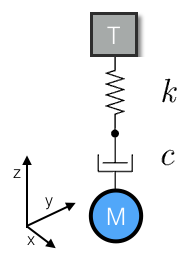
\includegraphics[width=0.32\textwidth]{illustrations/msd-1.png}
\caption{This illustration describes a basic mass-spring-damper system with spring constant $k$ and damping constant $c$. \label{illus:1}}
\end{figure}

\section{Physics of Multi-Dimensional Spring Systems}
As an introduction, we first describe the physics of a multi-dimensional spring system. This will provide the basic intuition for the deformable sheet model in the next section.
Figure \ref{illus:1} illustrates the most basic multi-dimensional spring system. A point mass $m$ is connected by a spring and damper to a infinitely strong block $T$. The spring constant is $k$ (let $\ell$ denote the resting length) and the damping constant is $c$. Let denote the acceleration vector $\mathbf{a} =  [ \ddot{x} ~~ \ddot{y} ~~ \ddot{z} ]^T$ of the point mass: 
\[
m \mathbf{a} = F_{spring} + F_{damper}.
\]
Hooke's law states that the magnitude of the force applied by a spring is proportional to its deviation $D$ from the rest length:
\[
|F_{spring}| = k D .
\]
Using unit vector notation, we can parametrize the force vector with spherical coordinates:
\[
F_{spring} =  ~\mathbf{i}~ k (D - \ell) \sin \theta \cos \psi +  ~\mathbf{j}~ k (D - \ell) \sin \theta \sin \psi + ~ \mathbf{k}~ k (D - \ell) \cos \theta 
\]
where $D = \sqrt{ (x-T_x)^2 + (y-T_y)^2 + (z-T_z)^2} $, $\theta = \cos^{-1} \frac{(z - T_z) }{D} $, $\psi = \tan ^{-1} \frac{(y - T_y) }{(x - T_x)}$.
For the damper, let $\mathbf{v} =  [ \dot{x} ~~ \dot{y} ~~ \dot{z} ]^T$ denote the velocity vector:
\[ F_{damper} = c \mathbf{v} .\]
The resulting equations of motion are:
\begin{equation}\footnotesize \selectfont
   m \mathbf{a} = ~\mathbf{i}~ (k (D - \ell) \sin \theta \cos \psi + c \mathbf{v}_x) +  ~\mathbf{j}~ (k (D - \ell) \sin \theta \sin \psi + c \mathbf{v}_y) + ~ \mathbf{k}~ (k (D - \ell) \cos \theta + c \mathbf{v}_z).
\end{equation}



\section{Simulator}
We can use this model to design a simulator for cutting deformable sheets.
Let $G_{x,y,z} \subset \mathbf{R}^3 $ be a three-dimensional global coordinate frame. 
We denote the set of points on this sheet as $\Sigma$, and $\Sigma^{(G)}$ is the locations of these points in the global frame.
The points are connected by a graph of springs and dampers.
To apply the above equation of motion, we can treat each neighboring vertex as a wall.
For each $p \in \Sigma$, the neighboring vertex $q \in N(p)$ applies a force $F_{pq}$. 
Cutting is modeled as removing an edge from the graph.
In this paper, we assume that all of the springs have the same constant, natural length, and all the damping constants are the same.

The simulator is initialized with some initial state $\Sigma^{(G)}_0 \in G_{x,y,z}$. 
The state is then iteratively updated based on the derived equations of motion above.
For each $p \in \Sigma$, the updates have the following form:
%Interaction between the vertices is governed by:
\begin{align}
\label{eq:vertex}
m \ddot{p}  = \sum_{q \in N(p)} F_{pq} + F_{external}
\end{align}
To update the position $p$, we use the implicit Adams method with a standard python toolkit \footnote{https://docs.scipy.org/doc/scipy-0.14.0/reference/generated/scipy.integrate.ode.html}. Tensioning is simulated as a position constraint for a chosen pinch point $p' \in \Sigma$:
\[
p' = u
\]
This means that regardless of the forces applied to this point it will remain at position $u$.

\section{Problem Statement}
We are given a rectangular planar sheet and a simple algebraic desired cutting contour of bounded curvature, which can be either closed or open.

\subsection{Cutting}
We assume that one arm of the robot is designated as the cutting arm and the other as the tensioning arm. A cutting contour is a sequence of points $C$ on the surface of the sheet. The cutting arm operates in an open-loop trajectory that attempts to cut along $C_0$, the position of the cutting contour in the global frame at time zero.
Error is measured using the symmetric difference between the desired contour on the sheet and the achieved contour cut. These will be different due to deformation of the sheet during cutting.
Let $X$ be the set of points inside a closed intended trajectory and let $Y$ be the set of points inside a closed simulated trajectory. The symmetric difference is then the exclusive-or $A \oplus B$ of the two sets. For open contours, the contours are closed by forming boundaries with the edges of the sheet.

\subsection{Tensioning}
Since the cutting is open-loop it cannot account for deformation, and this is why we need tensioning to apply feedback based on the state of the sheet.

\begin{definition}[Tensioning]
Let $s \in \Sigma$ be called a pinch point. 
Tensioning is defined as constraining the position of this pinch point to a specific location $u \in G_{x,y,z}$:
\[
T = \langle s, u \rangle
\]
\end{definition}

For each of the $k$ tensioning arms of the robot, we can have one tuple $T_i$. We consider a single pinch point for each arm for an entire cutting trajectory. This allows us to define a tensioning policy:

\begin{definition}[Tensioning Policy]
For arm $i\in \{1,..,k\}$, let $\Sigma^{(G)}_t$ be the locations of all of the points on the sheet in the global coordinate frame at time $t$. For a fixed pinch point $s$, a tensioning policy $\pi_s$ is a function where $\Delta_u = u_{t+1} - u_{t}$:
\[
\pi_i: \Sigma^{(G)}(t) \mapsto \Delta_u
\]

\end{definition}

\vspace{0.5em} \noindent\emph{Problem. Tensioning Policy Search: } For each arm $i$, find a tensioning policy that minimizes the symmetric difference of the desired vs. actual contour. 

\section{Reinforcement Learning For Policy Search}
We chose an RL algorithm since the symmetric difference reward function is non-convex and the system in non-linear.
We model the tensioning problem as a Markov Decision Process (MDP):
\[
\langle S,A,\xi(\cdot,\cdot), R(\cdot,\cdot),T \rangle.
\]
where the actions $A$ are 1$mm$ movements of the tensioning arm in the $x$ and $y$ directions, and the states $S$ are described below. The action space is tuned so the policy can generate sufficient tension to manipulate the cloth significantly over a few timesteps.  
Reward is measured using the symmetric difference between the desired contour and the achieved contour cut.
The robot receives 0 reward at all time-steps prior to the last step, and at the last time-step $T-1$ receives the symmetric difference. We do not shape the reward, as symmetric difference is exactly the error metric used for evaluation as well.

To optimize $\theta$, we leverage the TRPO implementation \cite{schulman2015trust} in Rllab \cite{duan2016benchmarking}. 
We use a neural network to parametrize the policy $\pi_\theta$, which maps an observation vector to a discrete action.
A two 32x32 Hidden Layer Multi-Layer Perceptron is used to represent this mapping. Since neural networks are differentiable, we can optimize the quantity $R(\theta)$.
The state space is a tuple consisting of the time index of the trajectory $t$, the displacement vector from the original pinch point $u_t$, and the location $x_i \in \mathbb{R}^3$ of fiducial points chosen randomly on the surface of the sheet. In all experiments we use $12$ fiducial points. 
This is a sample-based approximation of tracking $\Sigma^{(G)}_t$.


\section{Model-based Initialization}
Directly applying the RL algorithm to the FEM simulator has a two problems: (1) large sample complexity and (2) local minima.
Even in an optimized simulator, every new contour required 5 minutes of learning before a viable policy was found.
The key insight was that ultimately the simulator used in RL was based on an analytic model.
Thus, we explored whether we could initialize learning with a prior developed from a simplified objective.

\subsection{Small Deviation Approximation}
The equation of motion defines a non-linear system. We are, however, modeling point masses on a sheet that will have relatively small deformations from the resting length. 
We further assume that there is no damping $c=0$ or external forces.
For linearization, it is more convenient to work in Cartesian coordinates, so we can also re-parametrize the equations using Pythagorean identities:
\[
m a_x = k  \Delta_x - k \frac{\ell \Delta_x }{\sqrt{\Delta_x^2 + \Delta_y^2 + \Delta_z^2}} 
\]
\[
m a_y = k  \Delta_y - k \frac{\ell \Delta_y }{\sqrt{\Delta_x^2 + \Delta_y^2 + \Delta_z^2}}  
\]
\[
m a_z = k  \Delta_z - k\frac{\ell \Delta_z }{\sqrt{\Delta_x^2 + \Delta_y^2 + \Delta_z^2}} 
\]

To linearize, we can first take the gradient:
\[
\nabla(m a_x) = k \begin{bmatrix}
    1 - \frac{\ell (\Delta_y^2 + \Delta_z^2) }{(\sqrt{\Delta_x^2 + \Delta_y^2 + \Delta_z^2}) ^\frac{3}{2}} \\
    \frac{\ell \Delta_x \Delta_y }{(\sqrt{\Delta_x^2 + \Delta_y^2 + \Delta_z^2}) ^\frac{3}{2}} \\
    \frac{\ell \Delta_x \Delta_z }{(\sqrt{\Delta_x^2 + \Delta_y^2 + \Delta_z^2}) ^\frac{3}{2}} \\
\end{bmatrix} 
\]
We linearize around the operating point $\Delta_x, \Delta_y,\Delta_z = \rho = \frac{\ell}{\sqrt{3}}$, and let $\lambda = \frac{1}{3}\ell^{\frac{3}{2}}$:
\[
m a_x \approx  k \begin{bmatrix}
    1 - 2 \lambda \\
    \lambda \\
    \lambda \\
\end{bmatrix}^T \cdot \begin{bmatrix}
    (\Delta_x - \rho) \\
    (\Delta_y - \rho)\\
    (\Delta_z - \rho) \\
\end{bmatrix}, m a_y \approx  k \begin{bmatrix}
    \lambda \\
    1-2\lambda \\
    \lambda \\
\end{bmatrix}^T \cdot \begin{bmatrix}
    (\Delta_x - \rho) \\
    (\Delta_y - \rho)\\
    (\Delta_z - \rho) \\
\end{bmatrix}, m a_z \approx  k \begin{bmatrix}
    \lambda \\
    \lambda \\
    1-2\lambda \\
\end{bmatrix}^T \cdot \begin{bmatrix}
    (\Delta_x - \rho) \\
    (\Delta_y - \rho)\\
    (\Delta_z - \rho) \\
\end{bmatrix}
\]
We can define some notation to make the future algebra more concise:
\[
\mathbf{L} = \frac{k}{m} \begin{bmatrix}
   1- 2\lambda & \lambda & \lambda  \\
    \lambda & 1- 2\lambda & \lambda \\
    \lambda & \lambda  & 1-2\lambda \\
\end{bmatrix}
\]
The resulting system can be described in the state-space model for a position of a point mass $p$:
\begin{equation}
\ddot{p} = \mathbf{L} (\sum_{q \in N(p) }  (p - q) - \rho)
\end{equation}

\subsection{Tensioning Problem}
The key trick to understanding tensioning based on this linearization is an efficient computation of the equilibrium state, i.e., $\ddot{p} = 0$.
Let $X \in \mathbb{R}^{N \times 3}$ denote the positional state of each of the masses.
For $N$ masses and $E$ edges, let $A$ be an $E \times N$ matrix where every $A_{ij} = 0$ if edge i is not incident to the mass $j$, $A_{ij} = \pm 1$ for edges incident to the mass (pushing or pulling, can be selected arbitrarily).
And, finally, let $R$ be an $\mathbb{R}^{E \times 3}$ matrix where each component is $\rho$, or the natural length of the spring.
It can be shown that the acceleration of all of the masses is:
\[
\ddot{\mathbf{P}} =  A^T A X L - A^T R L 
\]
making the equilibrium condition:
\[
 A^T A X  =  A^T R 
\]

To enforce constraints, we simply have to enforce that some subset of the components of $X$ are fixed.
This restricts the equilibrium solution to the subspace of values for which $X_{i,:} = u_i$.
These are exactly the tensioning constraints, and we can solve the system of equations by partitioning the masses into free and tensioned sets.

First, we can re-write the above equation as:
\[
B X =  A^T R
\]
which can in turn be written as:
\[
B_{free} X_{free}  = A^T R + B_{tens} U
\]
and solving for the least squares solution
\[
X_{free}  = (B_{free}^T B_{free})^{-1} [B_{free}^T A^T R + B_{free}^T B_{tens} U]
\]
This expression is just an affine function of the tensioning constraints:
\[
X_{free}  = C U + D
\]

\begin{figure*}[t]
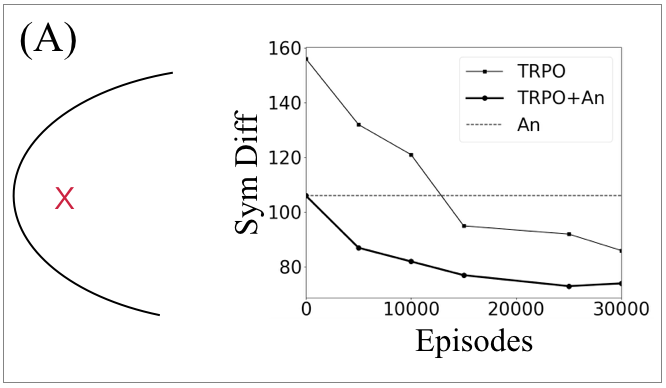
\includegraphics[width=0.32\textwidth]{figs/trpo-full-a.png}
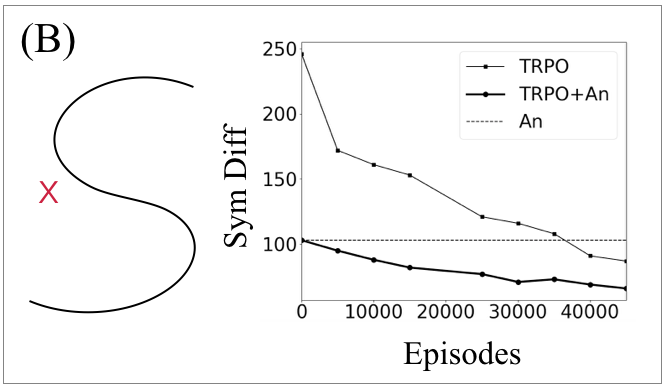
\includegraphics[width=0.32\textwidth]{figs/trpo-full-b.png}
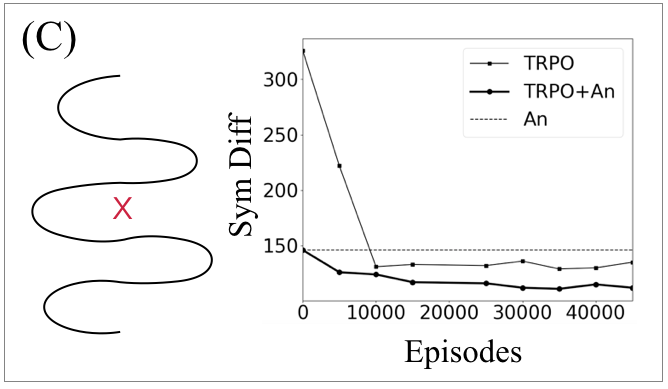
\includegraphics[width=0.32\textwidth]{figs/trpo-full-c.png}
\caption{This plot shows the expected reward over 50 trials for TRPO, TRPO initialized with the analytic approximation (TRPO AN), and the analytic model on its own. Three cutting curves are visualized of increasing difficulty with a single pinch point marked in red. Results suggest that initializing with an analytic model can greatly accelerate learning.\label{fig:1}}
\end{figure*}

\subsection{Optimization}
To find tensioning directions and magnitudes, we have to pose an optimization problem to set the values of U as the grid is cut.
The model and its equilibrium states give us a way to quantify deformation induced by cutting.
$C$ and $D$ depend on the structure of the graph at time $t$.

We cannot directly optimize for symmetric difference so instead, we optimize for minimizing total deformation from the original state:
\[ I_{t} =  \| X_{free}[0] - X_{free}[t+1] \|^2_2 \]
This measures the amount of change in the position of the points after a cut and the sheet has settled into a new equilibrium state.
This sets up our control objective for synthesizing a set of tensions from a fixed pinch point. 
\begin{equation}
   \min_{u_1,...,u_T} \sum_{t=0}^{T-1} I_{t} + q \|u_{t+1} - u_t \|_2^2  \label{obj}
\end{equation}
where $q \|u_{t+1} - u_t \|^2_2$ is a control penalty on changing the tensioning between time-steps for $q > 0$. 


This problem is a convex program which can be solved with standard solvers.
Once this open-loop strategy is learned, we can initialize TRPO by training the policy network to predict $u_{t}$ from the state.
Out intuition is that this analytic model gets close to the optimal policy and TRPO simply has to refine it.
This mitigates the effects of bad local minima far from the optimum and slow convergence.

\section{Results}
We present a set of illustrative initial experiments in this paper.
In the first experiment, we generated three contours of increasing difficulty and learned tensioning policies for a single pinch point $k=1$.
We compare TRPO with no initialization, TPRO+An with the analytic initialization, and An which is just the analytic model.
Figure \ref{fig:1} plots the learning curves.
We stopped training when the reward was no longer reliably decreasing.
We find that in all three cases, the analytic initialization significantly reduces the time needed to learn a similarly successful policy.
Furthermore, the analytic model is within 25\% of the final reward of TRPO achieves indicating that it is a very good initialization.

The next experiment evaluates the run time of the algorithms as we increase the number of tensioning arms.
Figure \ref{fig:2}A measures the number of episodes needed for TRPO to crossover, i.e., match the performance of the analytic method, as a function of the number of tensioning arms to plan for.
While the analytic method is greedy, TRPO requires nearly 350000 episodes before it is at parity with this method for 4 tensioning arms.
For comparison, the analytic optimization requires two orders of magnitude less time to reach the same result (Figure \ref{fig:2}B).
And, we explore using the combination of the two to achieve higher accuracy results with less rollouts.

\begin{figure}[ht]
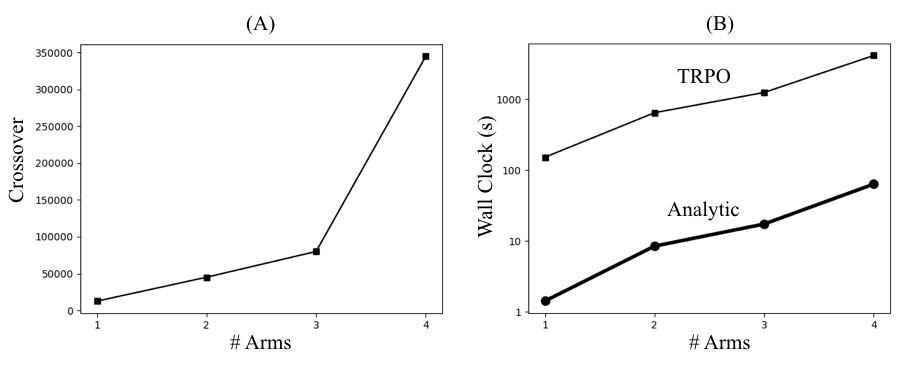
\includegraphics[width=\columnwidth]{figs/trpo-6.png}
\caption{(A) We measure the number of episodes needed for TRPO to crossover, i.e., match the performance of the analytic method, as a function of the number of tensioning arms to plan for. (B) For comparison, we plot the wall clock time of TRPO and the analytic optimization on a log scale. The optimization is order of magnitudes faster, but may be suboptimal. \label{fig:2}}
\end{figure}